\documentclass{article}
\usepackage{pdfpages}
\usepackage{hyperref}

\title{Team Liza \\ Milestone 2 \\ CSSE 374}
\author{Sam Kim \\ Kevin Geisler \\ Michael Williamson \\ Brian Collins}
\date{12/16/11}

\begin{document}

\maketitle
\newpage

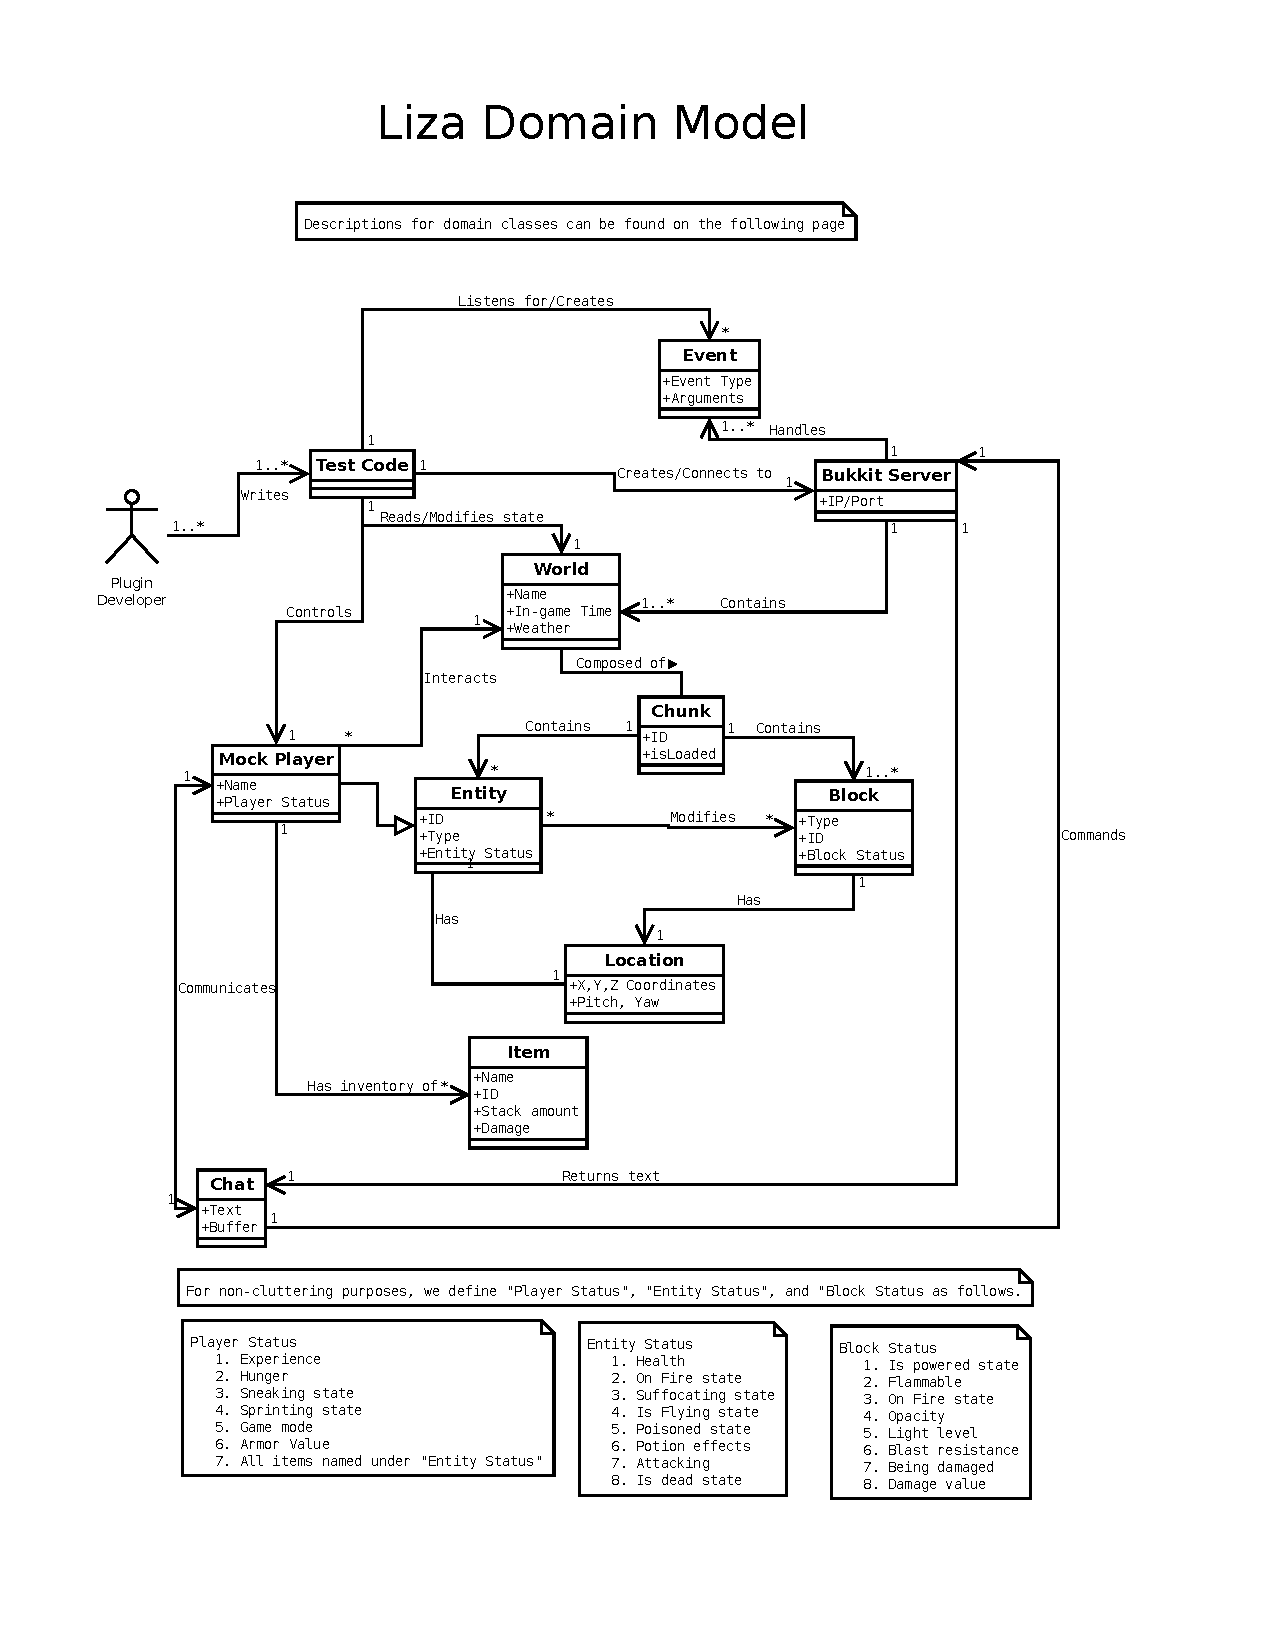
\includepdf[pages={-}]{Milestone2.pdf}

\section*{Domain Class Descriptions}

\subsection*{Actor}

This represents the Bukkit plugin developer. He/she writes and runs the
test code using Liza's API.

\subsection*{Test Code}

This is the code that contains the test cases written by the developer. 

\subsection*{Bukkit Server}

This is the instance of the server that Liza creates when running a test.
The most relevant data about the server is the Minecraft world it contains,
which is represented through associations.

\subsection*{Event}

As a game, most interactions are event driven. These are handled by
Minecraft with an internal Event Handler. Liza should be able to read these
events and create them.

\subsection*{World}

Represents the environment that a Minecraft player can interact with. 

\subsection*{Chunk}

The World is broken up into manageable pieces called chunks.

\subsection*{Block}

These make up the majority of the Minecraft world. There are blocks
of many types, such as stone, wood, sand, etc. These can be destroyed,
picked up by a player, and placed elsewhere.

\subsection*{Entity}

An Entity in Minecraft is anything in the world that isn't a block. This 
includes players and creatures.

\subsection*{Mock Player}

This represents the automated player which is controlled by Liza which will 
perform the actions defined by the plugin developer.

\subsection*{Location}

These are the coordinates in the Minecraft World

\subsection*{Item}

Items are things found in a player's inventory. 

\subsection*{Chat}

Players can communicate in the chat. Additionally, players can send commands
which are read by the server or a plugin. Typically, a command sends a response
back to the user. Liza will use this to assert that commands were sent properly.

\newpage

\section*{Action Items, Journal, and Project Plan}

These are found in our GoogleDocs pages

\href{https://docs.google.com/spreadsheet/ccc?key=0AjcjuiCChut1dGtnWlJqenU4ZDVENVdqUF9MWXVUWkE&hl=en_US#gid=0}{Project Plan}

\href{https://docs.google.com/document/d/1CwvcygEuj-zBrKCGxQtA8553bFEjGDdcFIdGDqVEmtA/edit?hl=en_US}{Journal and Action Items}

\end{document}